\documentclass[../DoAn.tex]{subfiles}
\usepackage{graphics}
\usepackage{float}
\begin{document}

\section{Khảo sát hiện trạng}
\label{section:2.1}
Khảo sát của Carousell\cite{carousell} - Tập đoàn chủ quản của Chợ Tốt cho thấy 72$\%$ trong số những người được phỏng vấn ở 8 quốc gia đã từng mua hàng second-hand. Tỷ lệ này thay đổi theo từng quốc gia, nhưng hầu hết đều ở mức trên 75$\%$, chỉ trừ Myanmar là 59$\%$, cao nhất là Philipines 92$\%$, Việt Nam ở mức 83$\%$. Đồng thời cũng theo Carousell, tại Việt Nam, tỉ lệ ưa chuộng mua đồ điện tử (máy chụp hình, máy tính, điện thoại di động, máy tính bảng,...) là 65$\%$, còn tỉ lệ ưa chuộng bán đồ điện tử là 69$\%$.

Sau ảnh hưởng của dịch Covid 19 các quy định về giãn cách xã hội khiến xu hướng tiêu dùng thay đổi, bao gồm cả việc mua bán đồ cũ. Theo đó, “máy tính xách tay” và “máy tính để bàn” là hai từ khóa được tìm kiếm nhiều nhất trên Chợ Tốt. Giãn cách xã hội đã khiến số lượng người làm việc tại nhà gia tăng khiến cho nhu cầu sử dụng máy tính để làm việc từ xa cũng tăng lên đáng kể.

Theo số liệu thống kê đối với những người thường xuyên hoạt động trên trang Chợ Tốt ở Việt Nam trong thời gian từ năm 2018-2021 (trong đó năm 2020 không có số liệu vì chuyển đổi hệ thống) thì 2 ngành hàng luôn được quan tâm nhiều nhất là xe hơi và thiết bị điện tử. Chợ Tốt cũng chính là một trang mua bán đồ cũ được nhiều người sử dụng nhưng lại chưa được chuyên biệt hóa dẫn đến lan man và tương đối khó khăn khi tìm kiếm sản phẩm đối với người dùng có nhu cầu cụ thể. Ở Việt Nam hiện nay mới chỉ có website ok.Xe là trang thương mại điện tử chuyên về việc mua bán xe máy, chưa có trang web nào chuyên biệt về mặt hàng đồ điện tử. Do đó, bản thân em đã hình thành ý tưởng xây dựng một nền tảng mua bán đồ cũ dành cho mặt hàng công nghệ. 

Các chức năng chính của hệ thống trao đổi đồ cũ cần phải có bao gồm:
\begin{itemize}
    \item Phía Người dùng bình thường – Người mua bán (Trader):
    \begin{itemize}
        \item Đăng ký, đăng nhập tài khoản bằng email
        \item Đăng bán sản phẩm đồ công nghệ cũ
        \item Tìm kiếm, xem, lưu bài đăng của người khác
        \item Quản lý bài đăng của cá nhân
        \item Quản lý thông tin cá nhân
        \item Báo cáo xấu bài đăng vi phạm
        \item Tương tác, trả giá sản phẩm bằng hình thức chat
    \end{itemize}
    \item Phía Quản trị viên (Admin):
        \begin{itemize}
        \item Quản lý người dùng
        \item Quản lý các báo cáo xấu vi phạm
        \item Xem thống kê của hệ thống
    \end{itemize}
\end{itemize}


\section{Tổng quan chức năng}

\subsection{Biểu đồ use case tổng quan}
\label{subsection:2.2.1}
Hệ thống được xây dựng phục vụ cho 3 tác nhân chính bao gồm: Khách (Guest), Người mua bán (Trader), Quản trị viên hệ thống (Admin). Với mỗi tác nhân, việc thực thi các ca sử dụng có sự khác biệt do phạm vi và quyền truy cập là khác nhau. Admin có vai trò quản lý người dùng và quản lý bài đăng, xem thống kê. Biểu đồ ca sử dụng tổng quan của toàn bộ hệ thống được mô tả như hình dưới đây:

\begin{figure}[h]
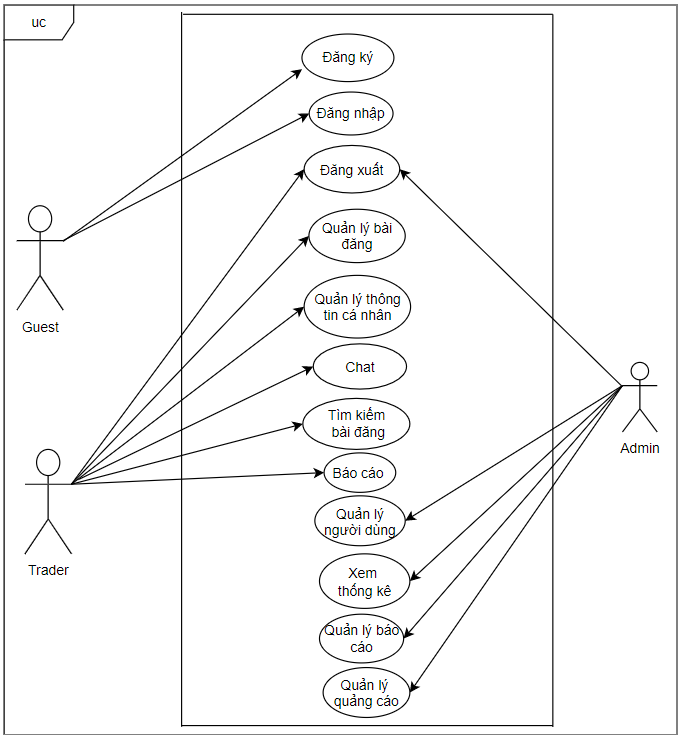
\includegraphics[width=0.75\linewidth]{Hinhve/overviewUsecase.png}
\centering
\caption{Biểu đồ use case tổng quan}
\end{figure}
\newpage

\subsection{Biểu đồ use case phân rã Quản lý bài đăng}
\label{subsection:2.2.2}

\begin{figure}[H]
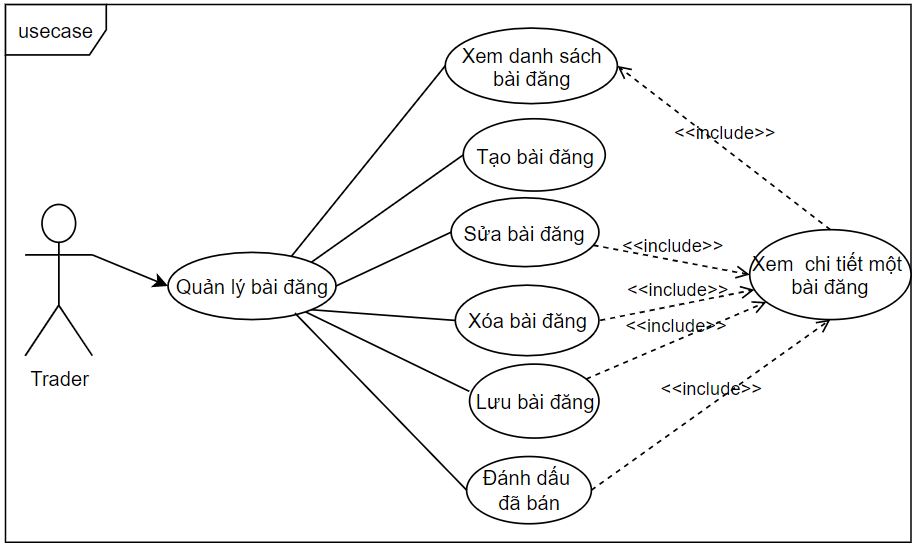
\includegraphics[width=0.75\linewidth]{Hinhve/PostManage.png}
\centering
\caption{Biểu đồ use case phân rã Quản lý bài đăng}
\end{figure}
Người dùng có thể sử dụng các chức năng trong Quản lý bài đăng là:
\begin{itemize}
\item Xem danh sách bài đăng: Người dùng vào mục cá nhân để xem danh sách các tin mình đã đăng.
\item Xem chi tiết một bài đăng: Từ danh sách bài đăng người dùng chọn và xem thông tin chi tiết của một bài đăng
\item Lưu bài đăng: Người dùng lưu thông tin một bài đăng của người khác mà mình quan tâm
\item Tạo mới bài đăng: Người dùng đăng 1 bài đăng mới bao gồm thông tin của mặt hàng và ảnh minh họa nếu muốn
\item Đánh dấu bài đăng là đã bán
\item Sửa bài đăng: Người dùng sửa thông tin bài đăng của mình đã đăng lên
\item Xóa bài đăng: Người dùng xóa bài đăng của mình đã đăng lên
\end{itemize} 
\newpage

\subsection{Biểu đồ use case phân rã Quản lý thông tin cá nhân}
\label{subsection:2.2.3}
\begin{figure}[H]
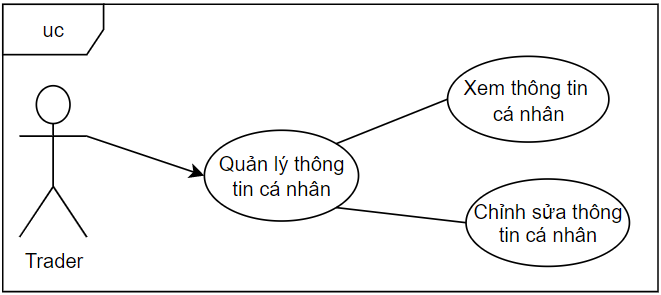
\includegraphics[width=0.75\linewidth]{Hinhve/profileManage.png}
\centering
\caption{Biểu đồ use case phân rã Quản lý thông tin cá nhân}
\end{figure}

Người dùng có thể sử dụng các chức năng trong Quản lý thông tin cá nhân là:

\begin{itemize}
\item Xem thông tin cá nhân: Người dùng xem thông tin cá nhân của bản thân hoặc của người dùng khác
\item Đổi thông tin cá nhân: Người dùng đổi  tên, số điện thoại hoặc thay đổi ảnh đại diện của bản thân 
\end{itemize}

\subsection{Biểu đồ use case phân rã Quản lý người dùng}
\label{subsection:2.2.4}
\begin{figure}[H]
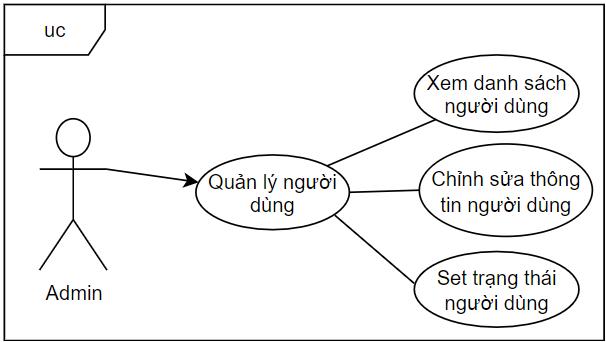
\includegraphics[width=0.75\linewidth]{Hinhve/userManage.png}
\centering
\caption{Biểu đồ use case phân rã Quản lý người dùng}
\end{figure}

Quản trị viên (Admin) có thể sử dụng các chức năng trong Quản lý người dùng là:

\begin{itemize}
\item Xem danh sách người dùng: Quản trị viên xem danh sách người có trong hệ thống
\item Chỉnh sửa thông tin người dùng: Quản trị viên lựa chọn và sửa thông tin của người dùng 
\item Thiết lập trạng thái người dùng: Quản trị viên thiết lập trạng thái hoạt động của người dùng
bao gồm active hoặc inactive
\end{itemize}

\subsection{Biểu đồ use case phân rã Quản lý báo cáo}
\label{subsection:2.2.5}
\begin{figure}[H]
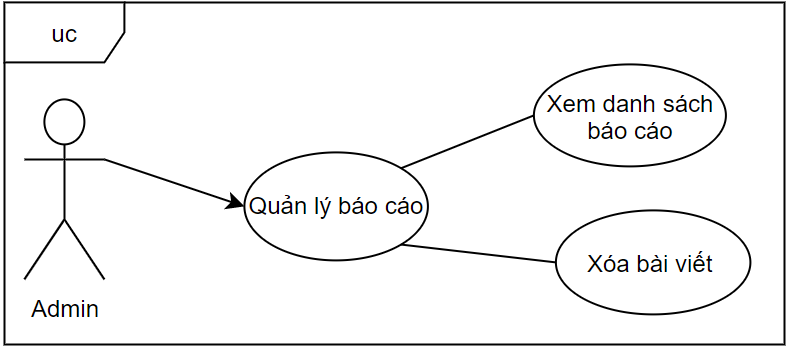
\includegraphics[width=0.75\linewidth]{Hinhve/ReportManage.png}
\centering
\caption{Biểu đồ use case phân rã Quản lý báo cáo}
\end{figure}

Quản trị viên (Admin) có thể sử dụng các chức năng trong Quản lý báo cáo là:

\begin{itemize}
\item Xem danh sách báo cáo: Quản trị viên xem danh sách các bài viết bị người dùng báo cáo
\item Xóa bài viết: Quản trị viên xóa bài viết bị cáo cáo nếu nội dung báo cáo là đúng
\end{itemize}

\subsection{Biểu đồ use case phân rã Quản lý quảng cáo}
\label{subsection:2.2.5}
\begin{figure}[H]
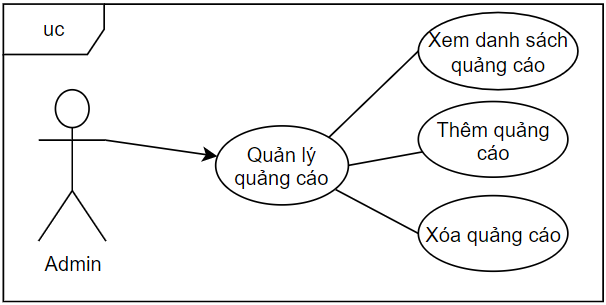
\includegraphics[width=0.75\linewidth]{Hinhve/adsManage.png}
\centering
\caption{Biểu đồ use case phân rã Quản lý quảng cáo}
\end{figure}

Quản trị viên (Admin) có thể sử dụng các chức năng trong Quản lý quảng cáo là:

\begin{itemize}
\item Xem danh sách quảng cáo: Quản trị viên xem danh sách quảng cáo đang được hiển thị ở trang chủ phía người dùng
\item Thêm quảng cáo: Quản trị viên thêm một quảng cáo mới
\item Xóa quảng cáo: Quản trị viên xóa một quảng cáo 
\end{itemize}
\subsection{Quy trình nghiệp vụ}
\label{subsection:2.2.3}
Hệ thống có một quy trình nghiệp vụ quan trọng nhất chính là quy trình mua bán đồ cũ, bao gồm các bước sơ bộ như sau:

\begin{enumerate}
\item Cả người mua và người bán đều cần phải đăng ký tài khoản trên thống
\item Người bán đăng sản phẩm kèm thông tin sản phẩm, giá bán
\item Người mua tìm kiếm thông tin sản phẩm trên hệ thống
\item Người mua tìm thấy sản phẩm và bắt đầu nhắn tin hỏi chi tiết về sản phẩm, thương lượng về giá cả với người bán thông qua hệ thống chat được tích hợp trên hệ thống
\item Người mua và người bán hẹn nhau mua bán trực tiếp hoặc chuyển phát
\item Nếu giao dịch thành công người bán sẽ đánh dấu bài đăng thành trạng thái đã bán
\end{enumerate}
\newpage

\section{Đặc tả chức năng}
\label{section:2.3}
\subsection{Đặc tả use case Quản lý bài đăng
}
\hfill
% Please add the following required packages to your document preamble:
% \usepackage{booktabs}
\begin{table}[H]
\begin{tabular}{|p{3cm}|p{12cm}|}
\hline
Use case ID         & UC01                                                                                                               \\ \hline
Tên use case        & Quản lý bài đăng                                                                                                   \\ \hline
Tên tác nhân        & Người dùng                                                                                                         \\ \hline
Mô tả               & Ca sử dụng cho phép người dùng tương tác với bài đăng                                                              \\ \hline
Tiền điều kiện      & Người dùng đã đăng nhập, tồn tại bài đăng tương ứng                                                                                                              \\ \hline
Hậu điều kiện       & Thao tác thành công                                                                                                              \\ \hline
Luồng sự kiện chính & 
\begin{itemize}
\item Ca sử dụng bắt đầu khi người dùng truy cập vào hệ thống và xem danh sách bài đăng, chọn xem chi tiết một bài đăng (nếu muốn)
\item Người dùng chọn sử dụng các thao tác:
\begin{itemize}
\item Tạo mới bài đăng của bản thân
\item Chỉnh sửa bài đăng của bản thân
\item Lưu bài bài đăng cửa người khác
\item Đánh dấu bài đăng của bản thân đã được bán
\item Xóa bài đăng của bản thân
\end{itemize}
\end{itemize} \\\hline
Luồng sự kiện phụ   &                                      \begin{itemize}
\item Tạo mới bài đăng của bản thân
\begin{itemize}
\item Người dùng nhập thông tin về bài đăng và xác nhận
\item Hệ thống thông báo trạng thái và lưu thông tin bài đăng
\end{itemize}
\item Chỉnh sửa bài đăng của bản thân
\begin{itemize}
\item Người dùng chỉnh sửa thông tin về bài đăng và xác nhận
\item Hệ thống thông báo trạng thái và cập nhật thông tin bài đăng
\end{itemize}
\item Lưu bài bài đăng cửa người khác
\begin{itemize}
\item Lựa chọn và lưu bài đăng muốn xem sau
\item Hệ thống thông báo trạng thái và lưu bài đăng vào danh sách bài đăng đã lưu của người dùng
\end{itemize}
\item Đánh dấu bài đăng của bản thân đã được bán
\begin{itemize}
\item Lựa chọn và đánh dấu bài đăng đã được bán
\item Hệ thống thông báo trạng thái và lưu bài trạng thái bài đăng
\end{itemize}
\item Xóa bài đăng của bản thân
\begin{itemize}
\item Lựa chọn và xác nhận xóa bài đăng
\item Hệ thống thông báo trạng thái và lưu bài trạng thái bài đăng
\end{itemize}
\end{itemize}                                 \\ \hline
Ngoại lệ            & Xuất hiện lỗi, Hệ thống thông báo lỗi tương ứng với thao tác                                                                                             \\ \hline
Tần suất sử dụng    & Cao                                                                                                                \\ \hline
\end{tabular}
\caption{Đặc tả use case Quản lý bài đăng}
\label{tab:my-table}
\end{table}
\newpage
\subsection{Đặc tả use case Quản lý bài đăng
}
\hfill
% Please add the following required packages to your document preamble:
% \usepackage{booktabs}
\begin{table}[H]
\begin{tabular}{|p{3cm}|p{12cm}|}
\hline
Use case ID         & UC02                                                                                                               \\ \hline
Tên use case        & Quản lý thông tin cá nhân                                                                                                   \\ \hline
Tên tác nhân        & Người dùng                                                                                                         \\ \hline
Mô tả               & Ca sử dụng cho phép người dùng xem và chỉnh sửa thông tin cá nhân của mình                                                              \\ \hline
Tiền điều kiện      & Người dùng đã đăng nhập                                                                                                           \\ \hline
Hậu điều kiện       & Thao tác thành công                                                                                                              \\ \hline
Luồng sự kiện chính & 
\begin{itemize}
\item Ca sử dụng bắt đầu khi người dùng truy cập vào hệ thống và chọn chức năng quản lý thông tin cá nhân
\item Người dùng ban đầu có thể xem thông tin cá nhân và các bài đăng của mình. Sau đó gười dùng chọn sử dụng các thao tác:
\begin{itemize}
\item Cập nhật thông tin cơ bản như ảnh đại diện, tên, số điện thoại
\item Thay đổi mật khẩu đăng nhập
\end{itemize}
\end{itemize} \\\hline
Luồng sự kiện phụ   &                                      \begin{itemize}
\item Cập nhật thông tin cơ bản
\begin{itemize}
\item Người dùng nhập điền các thông tin cá nhân cần cập nhật và chọn xác nhận
\item Hệ thống thông báo trạng thái và cập nhật thông tin.
\end{itemize}
\item Thay đổi mật khẩu đăng nhập
\begin{itemize}
\item Người dùng nhập mật khẩu cũ và nhập mật khẩu mới để xác minh
\item Hệ thống kiểm tra xem mật khẩu cũ có trùng khớp với dữ liệu hay không sau đó thông báo trạng thái và cập nhật mật khẩu nếu mật khẩu cũ chính xác
\end{itemize}
\end{itemize}                                 \\ \hline
Ngoại lệ            & Xuất hiện lỗi, Hệ thống thông báo lỗi tương ứng với thao tác                                                                                             \\ \hline
Tần suất sử dụng    & Thấp                                                                                                                \\ \hline
\end{tabular}
\caption{Đặc tả use case Quản lý bài đăng}
\label{tab:my-table}
\end{table}
\newpage
\subsection{Đặc tả use case Tìm kiếm bài đăng}
\hfill
\begin{table}[H]
\begin{tabular}{|p{3cm}|p{12cm}|}
\hline
Use case ID         & UC03                                                                                                               \\ \hline
Tên use case        & Tìm kiếm bài đăng                                                                                                   \\ \hline
Tên tác nhân        & Người dùng                                                                                                         \\ \hline
Mô tả               & Ca sử dụng cho phép người dùng tìm kiếm bài đăng theo nhu cầu\\ \hline
Tiền điều kiện      & Không                                                                                                              \\ \hline
Hậu điều kiện       & Tìm kiếm bài đăng thành công                                                                                                              \\ \hline
Luồng sự kiện chính & 
\begin{itemize}
\item Ca sử dụng bắt đầu khi người dùng truy cập vào hệ thống và bắt đầu tìm kiếm
\item Người dùng chọn sử dụng các thao tác:
\begin{itemize}
\item Tìm kiếm bài đăng theo danh mục
\item Tìm kiếm bài đăng theo từ khóa
\end{itemize}
\end{itemize} \\\hline
Luồng sự kiện phụ   &                                      \begin{itemize}
\item Tìm kiếm bài đăng theo danh mục
\begin{itemize}
\item Người dùng chọn một danh mục hiển thị ở trang chủ
\item Hệ thống hiển thị danh sách bài đăng theo danh mục đã chọn
\end{itemize}
\item Tìm kiếm bài đăng theo từ khóa
\begin{itemize}
\item Người dùng nhập từ khóa sản phẩm cần mua vào ô tìm kiếm
\item Hệ thống hiển thị danh sách sản phẩm liên quan đến từ khóa đã nhập
\end{itemize}
\end{itemize}                                 \\ \hline
Ngoại lệ            & Không tìm thấy bài đăng phù hợp                                                                                             \\ \hline
Tần suất sử dụng    & Cao                                                                                                                \\ \hline
\end{tabular}
\caption{Đặc tả use case Tìm kiếm bài đăng}
\label{tab:my-table}
\end{table}
\newpage

\subsection{Đặc tả use case Chat}
\hfill
\begin{table}[H]
\begin{tabular}{|p{3cm}|p{12cm}|}
\hline
Use case ID         & UC04                                                                                                               \\ \hline
Tên use case        & Chat                                                                                                   \\ \hline
Tên tác nhân        & Người dùng                                                                                                         \\ \hline
Mô tả               & Ca sử dụng xuất hiện khi người dùng chọn chức năng chat để có thể hỏi thêm về thông tin sản phẩm, mặc cả giá\\ \hline
Tiền điều kiện      & Người dùng đã đăng nhập                                                                                                              \\ \hline
Hậu điều kiện       & Gửi và nhận tin nhắn thành công                                                                                                              \\ \hline
Luồng sự kiện chính & 
\begin{itemize}
    \item Ca sử dụng bắt đầu khi người dùng truy cập vào hệ thống, xem một bài đăng bất kì
    \item Người sử dụng chọn chức năng chat trong bài đăng
    \item Hệ thống hiển thị giao diện chat
    \item Người mua gửi tin nhắn cho người bán
    \item Hệ thống lưu thông tin tin nhắn và gửi đến cho người bán
    \item Người bán nhận được tin nhắn và phản hồi người mua
    \item Quá trình gửi và nhận tin nhắn có thể được lặp lại bởi người dùng
\end{itemize} \\\hline
Luồng sự kiện phụ   &                                      \begin{itemize}
    \item Người dùng chọn chức năng chat
    \item Chọn người muốn chat
    \item Hệ thống lấy lịch sử nói chuyện của 2 người và hiển thị 
    \item Người dùng thực hiện gửi tin nhắn
\end{itemize}                                 \\ \hline
Ngoại lệ            & Không có                                                                                            \\ \hline
Tần suất sử dụng    & Cao                                                                                                                \\ \hline
\end{tabular}
\caption{Đặc tả use case Chat}
\label{tab:my-table}
\end{table}
\newpage

\subsection{Đặc tả use case Báo cáo xấu}
\hfill
\begin{table}[H]
\begin{tabular}{|p{3cm}|p{12cm}|}
\hline
Use case ID         & UC05                                                                                                               \\ \hline
Tên use case        & Báo cáo xấu                                                                                                   \\ \hline
Tên tác nhân        & Người dùng                                                                                                         \\ \hline
Mô tả               & Ca sử dụng cho phép người dùng báo cáo bài đăng khi phát hiện thấy bài đăng hoặc người dùng có dấu hiệu sai sự thật, lừa đảo\\ \hline
Tiền điều kiện      & Người dùng đã đăng nhập                                      \\ \hline
Hậu điều kiện       & Báo cáo bài đăng thành công                                  \\ \hline
Luồng sự kiện chính & 
\begin{itemize}
    \item Ca sử dụng bắt đầu khi người dùng truy cập vào hệ thống, xem một bài đăng và có dấu hiệu vi phạm
    \item Người dùng nhấn nút báo cáo trong bài đăng
    \item Hệ thống hiển thị ô nhập thông tin báo cáo
    \item Người dùng nhập thông tin báo cáo
    \item Xác nhận gửi báo cáo
    \item Hệ thống lưu lại thông tin báo cáo và thông báo trạng thái cho người dùng
\end{itemize} \\\hline
Luồng sự kiện phụ   & Không có\\ \hline
Ngoại lệ            & Không có                                                                                            \\ \hline
Tần suất sử dụng    & Thấp                                                                                                                \\ \hline
\end{tabular}
\caption{Đặc tả use case Báo cáo xấu}
\label{tab:my-table}
\end{table}
\newpage

\subsection{Đặc tả use case Quản lý cáo xấu}
\hfill
\begin{table}[H]
\begin{tabular}{|p{3cm}|p{12cm}|}
\hline
Use case ID         & UC06                                                                                                               \\ \hline
Tên use case        & Quản lý báo cáo                                                                                                   \\ \hline
Tên tác nhân        & Quản trị viên                                                                                                         \\ \hline
Mô tả               & Ca sử dụng cho quản trị viên xem danh sách các bài viết bị báo cáo bởi người dùng\\ \hline
Tiền điều kiện      & Quản trị viên đã đăng nhập                                      \\ \hline
Hậu điều kiện       & Thực hiện thao tác thành công                                 \\ \hline
Luồng sự kiện chính & 
\begin{itemize}
    \item Ca sử dụng bắt đầu khi người quản trị viên đăng nhập vào hệ thống, hệ thống hiển thị giao diện quản trị
    \item Người quản trị viên lựa chọn chức năng Quản lý báo cáo
    \item Hệ thống hiển thị danh sách các bài đăng bị báo cáo
    \item Quản trị viên có thể xem bài đăng bị báo cáo và xóa bài đăng đó nếu muốn
\end{itemize} \\\hline
Luồng sự kiện phụ   & Không có\\ \hline
Ngoại lệ            & Không có                                                                                            \\ \hline
Tần suất sử dụng    & Thấp                                                                                                                \\ \hline
\end{tabular}
\caption{Đặc tả use case Quản lý báo cáo}
\label{tab:my-table}
\end{table}
\section{Yêu cầu phi chức năng}
\label{section:2.4}
Các yêu cầu phi chức năng của hệ thống bao gồm:
\begin{itemize}
    \item Các tình năng hoạt động ổn định, tốc độ phản hồi tốt.
    \item Phù hợp với các trình duyệt web khác nhau như chrome, cốc cốc,...
    \item Có khả năng đáp ứng các kích thước màn hình ở các thiết bị khác
nhau như điện thoại, máy tính,...
    \item Có khả năng cải tiến, phát triển tính năng mới.
    \item Giao diện thân thiện, đơn giản dễ sử dụng.
\end{itemize}


%%%%%%%%%%%%%%%%%%%%%%%%%%%%%%%%%%%

\end{document}